\documentclass[../main.tex]{subfiles}
\graphicspath{{\subfix{../figures/}}}

\begin{document}
\section{实验环境}
\begin{enumerate}
  \item Windows 操作系统 (指挥者): 作为实验环境中的主控制中心,负责与嵌入式系统进行交互,向其下达指令并监控实验的进行。
  \item ESP8266 WiFi 模块 (攻击实施者):
    担当实验中的攻击者,根据指挥者的指令执行相应的操作。
    其主要任务是模拟Deauth攻击,
    通过向无线网络中的设备发送Deauthentication帧来切断其网络连接,
    进而影响无线网络对用户的可用性。
\end{enumerate}

在这个实验环境中,Windows 操作系统扮演着指挥者的角色,通过与ESP8266 Wi-Fi
模块进行通信来控制实验的执行。ESP8266 Wi-Fi
模块则作为攻击实施者,在接收到指挥者的指令后,
执行Deauth攻击的操作,验证网络的弱点并评估其可用性受到的影响。
这样的实验设置有助于探究无线网络安全性与稳定性之间的关系,为网络防御提供重要参考。
%
\subsection{ESP8266 Wi-Fi 模块}
\begin{figure}[H]
  \begin{center}
    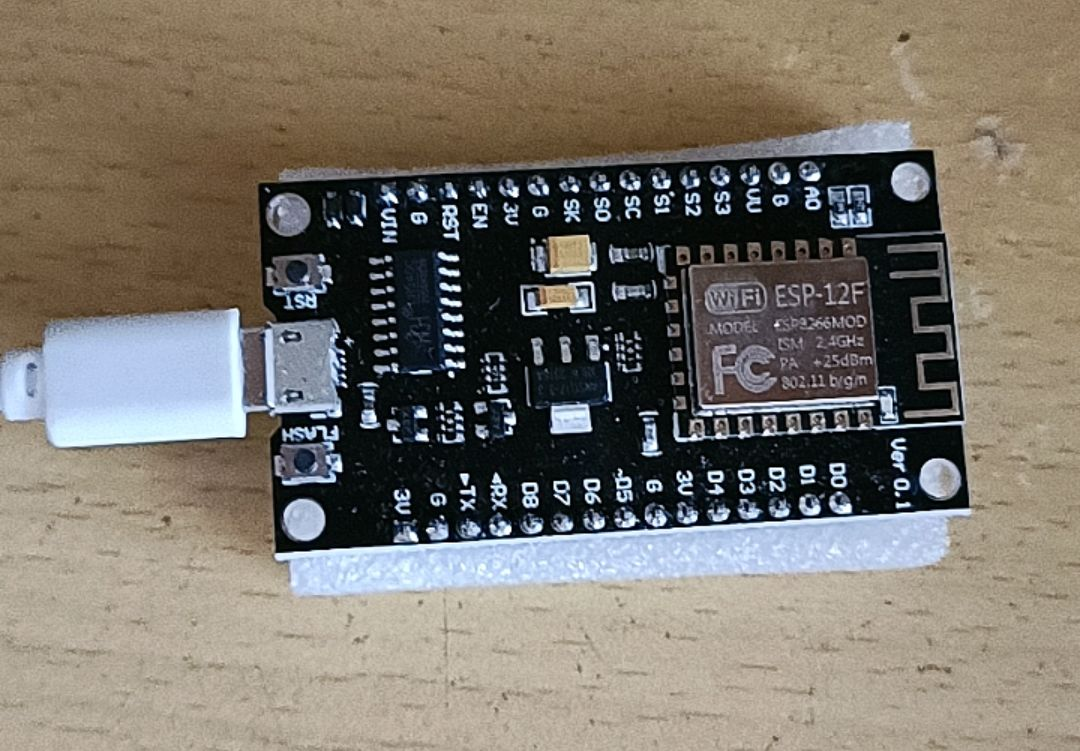
\includegraphics[width=0.20\textwidth]{esp8266.jpg}
  \end{center}
  \caption{ESP8266 Wi-Fi 模块}
\end{figure}

ESP8266 Wi-Fi 模块是一种低成本、高性能的Wi-Fi模块,由乐鑫(Espressif Systems)公司推出。
它基于Espressif的ESP8266芯片,提供了便捷的无线网络连接功能和灵活的用户程序功能。
ESP8266 具有小巧的尺寸,低功耗和强大的处理能力,适合于各种物联网应用和嵌入式系统项目。

ESP8266 Wi-Fi 模块支持802.11 b/g/n标准,能够实现可靠的无线连接,
并通过串口等接口与外部设备或主控制器进行通信。
它可以作为独立的Wi-Fi模块,也可以作为主控制器运行用户自定义的应用程序。

由于其强大的功能和良好的性价比,ESP8266 Wi-Fi 模块被广泛应用于物联网设备、
智能家居、智能设备、传感器网络等领域。开发人员可以利用其丰富的软件开发工具和社区支持,
快速开发出各种创新的无线网络应用。
\end{document}
